\jxhj{%教学后记
	}
\skrq{%授课日期
	2017年9月28日 4-5节}
\ktmq{%课题名称
	刀具半径补偿 }
\jxmb{%教学目标,每行前面要加 \item
	\item 了解补偿的意义;
	\item 掌握G41/G42刀具半径补偿指令的使用;
	\item 会用G41/G42刀具半径指令编写程序;
	\item 了解常用切入切出的方法。
}
\jxzd{%教学重点,每行前面要加 \item
	\item 掌握G41/G42刀具半径补偿指令的使用;
	\item 会用G41/G42刀具半径指令编写程序;}
\jxnd{%教学难点,每行前面要加 \item
	\item 会用G41/G42刀具半径指令编写程序;}
\jjff{%教学方法
	通过讲述、举例、演示法来说明;}

\makeshouye %制作教案首页

%%%%教学内容
\subsection{组织教学}
\begin{enumerate}[1、]
	\item 集中学生注意力;
	\item 清查学生人数;
	\item 维持课堂纪律;
\end{enumerate}
\subsection{复习导入及主要内容}
\begin{enumerate}[1、]
\item 在数控铣床或加工中心上加工如图所示的零件,试完成程序的编写。(试用I、J、K编写,凸台高5mm)

\begin{figure}[h]
	\centering
	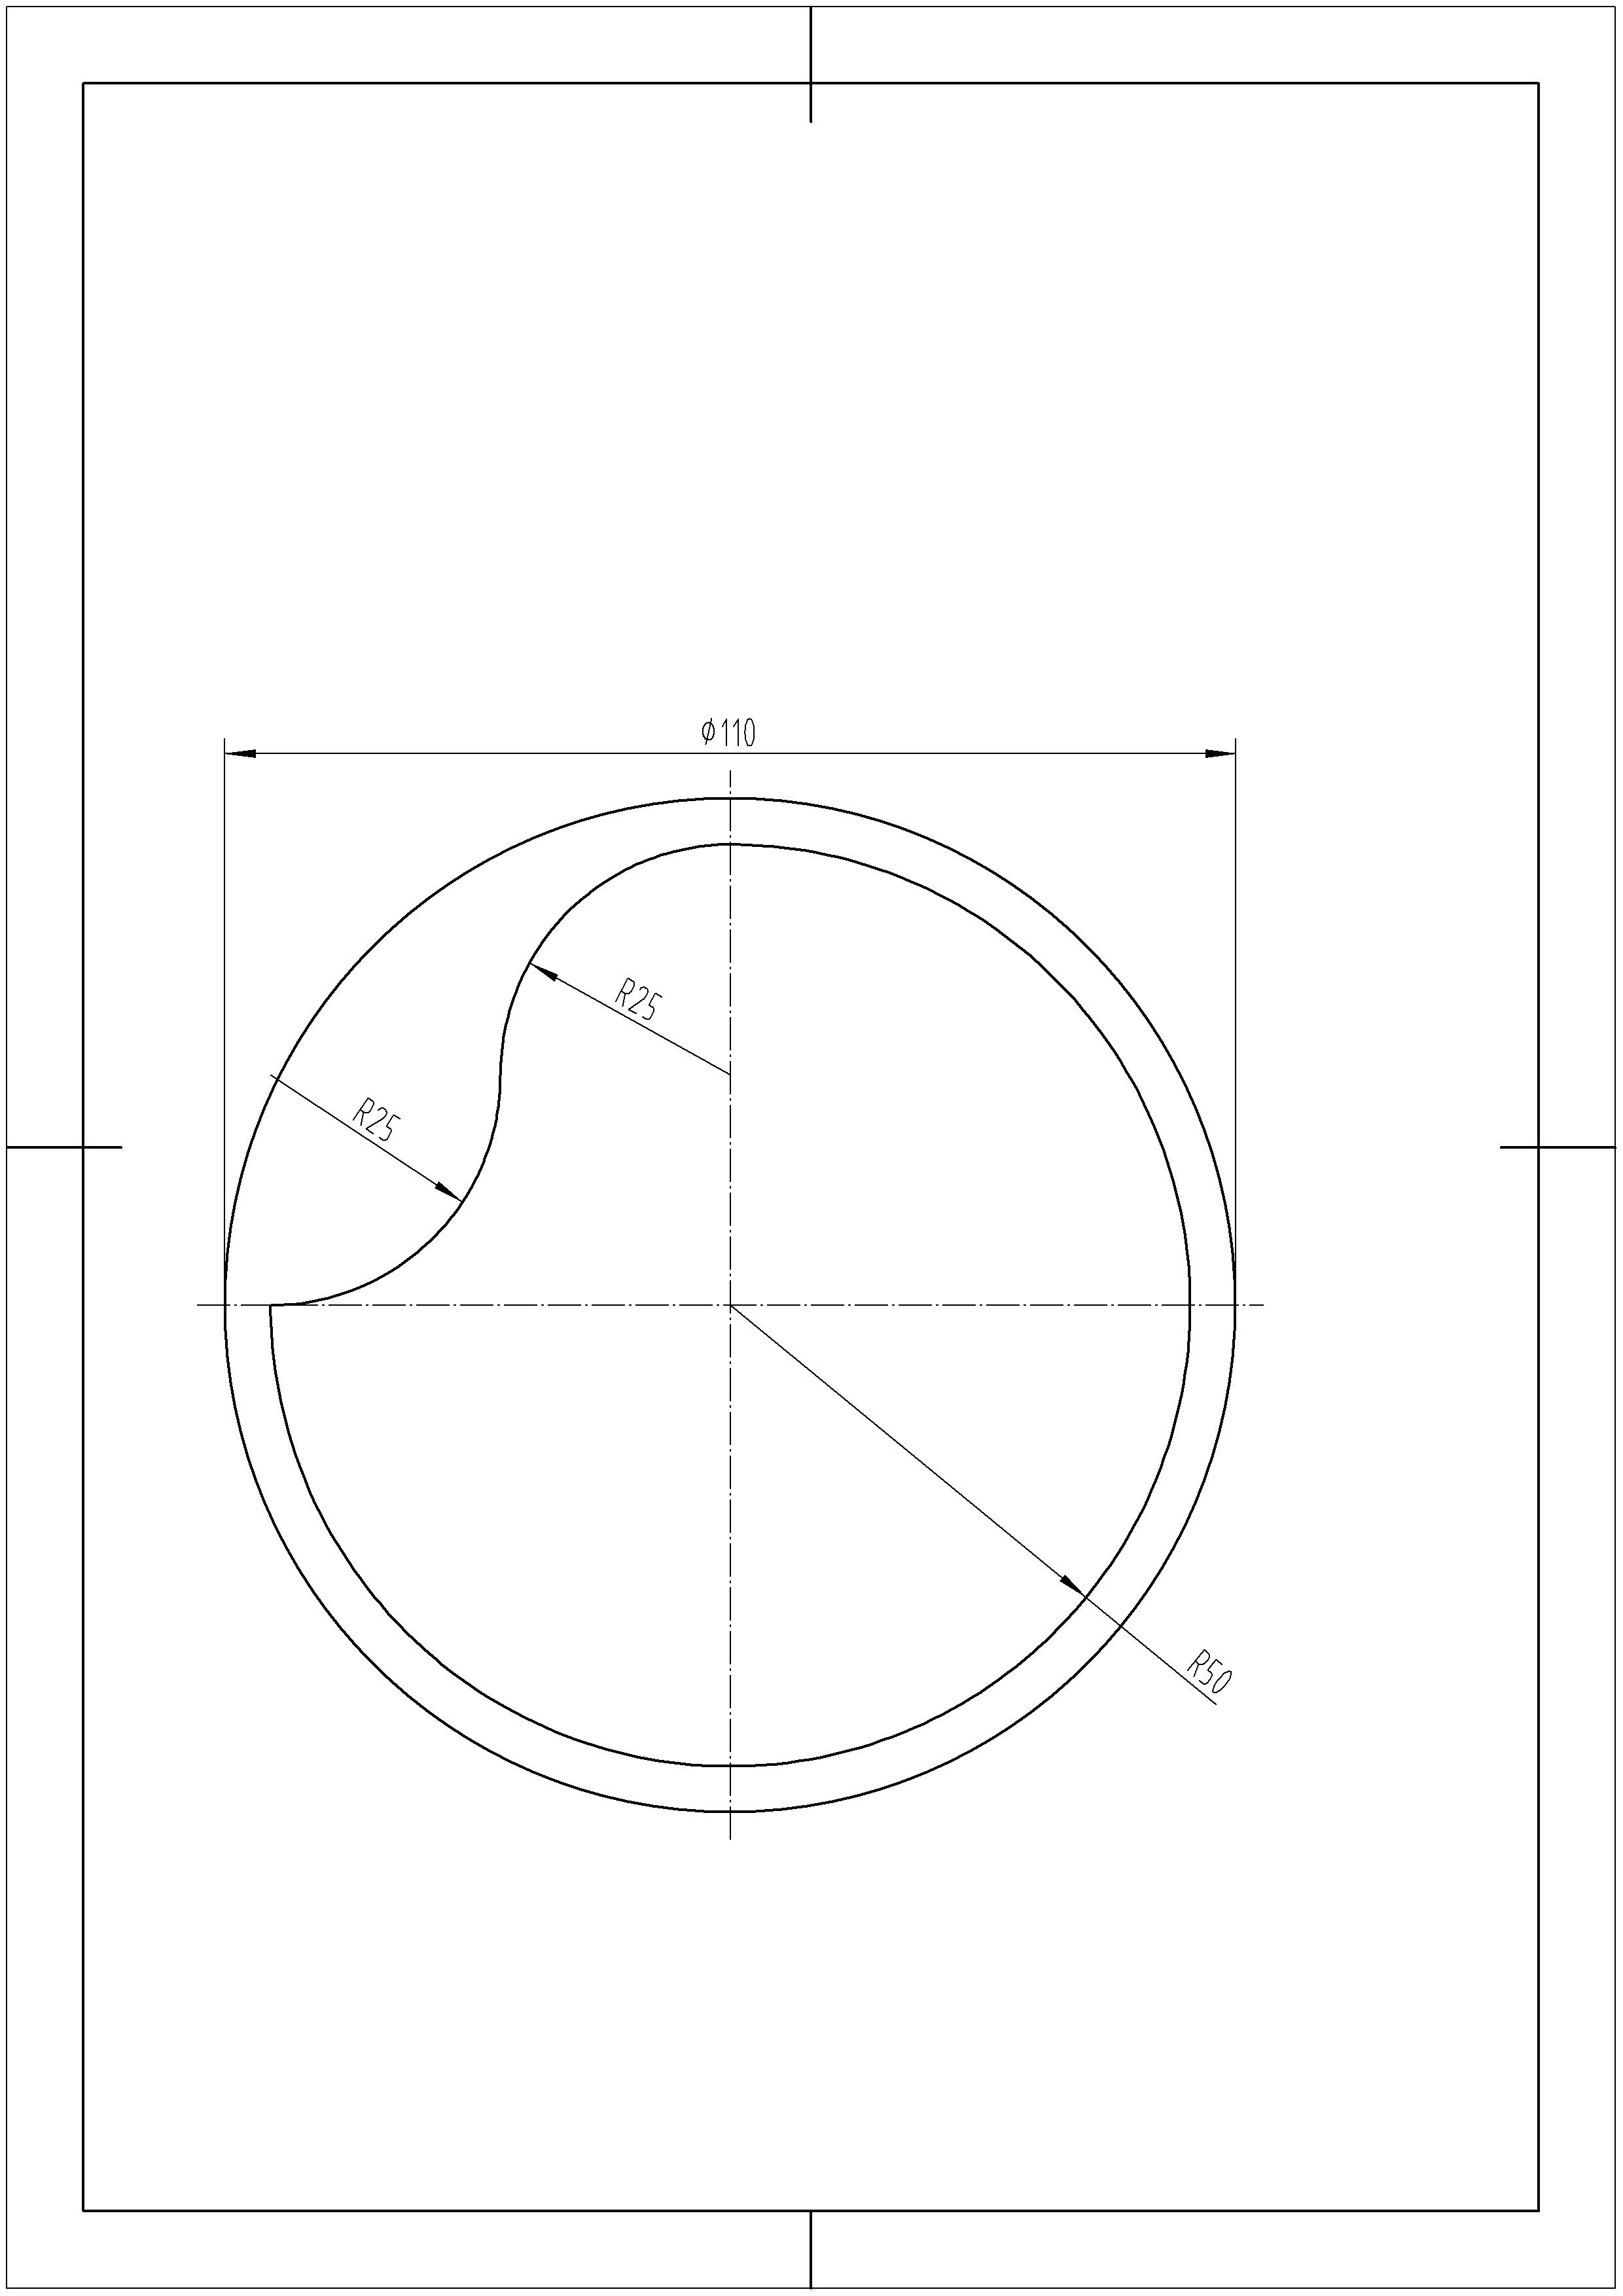
\includegraphics[width=0.8\linewidth,trim=40 150 70 220,clip]{data/image/7-1.jpg}
	\caption{复习题}
	\label{fig:7-1}
\end{figure}

\item G2/G3指令半径编程;
\item G2/G3指令圆心编程;
\item 编写程序的基本思路。
\end{enumerate}

\subsection{教学内容及过程}

\subsubsection{加工尺寸的分析}

由于加工刀具存在一个尺寸,故加工出来的尺寸值会每边少一个刀具半径。

解决方法:

1、更改加工刀路,使其偏移一个刀具半径(粗加工及去残料)。

2、使用刀具半径补偿指令进行编程。

例子:

\begin{lstlisting}
O0001;
G54G71G40G90;
M3S500;
G1Z30.F200O;
X70.YO;
Z5.;
Z-5.F200;
X66.Y10.;
G3X56.Y0R10.;
G2X-56.I-56.;
G2X-50.Y6.0.I6.0;(中间的过度)
G3X-31.Y25.J19.;
G2X0Y56.I31.;
X56.YOJ-56.;
G3X66.Y-10.I10.;
G1Z5.0;
Z30.F2000;
M5;
M30;
\end{lstlisting}
(麻烦,但有时必须这么做)


\subsubsection{刀具半径补偿}

由CNC系统内部使刀具在加工时,自动偏移一个刀具半径。
简化编程的难度。

指令G40、G41/G42

1、补偿方向的确定:

ISO 标准规定,当刀具中心轨迹在编程轨迹前进方向的左边时,称为左刀补,用G41表示;刀具中心轨迹在编程轨迹前进方向的右边时,称为右刀补,用G42表示;注销刀具半径补偿时用G40表示。

\begin{figure}[h]
	\centering
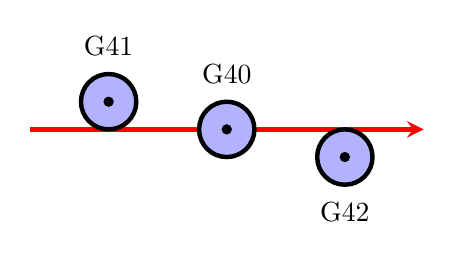
\begin{tikzpicture}[ultra thick]
\draw[->,red,>=stealth]  (0,0) -- (5,0);
\draw[fill=blue!30] (1,10pt) circle (10pt) circle (1pt);
\draw[fill=blue!30] (2.5,0) circle (10pt) circle (1pt);
\draw[fill=blue!30] (4,-10pt) circle (10pt) circle (1pt);
\node at (1,30pt) {G41};
\node at (2.5,20pt) {G40};
\node at (4,-30pt) {G42};
\end{tikzpicture}
\caption{刀补位置}
\label{fig:7-1}
\end{figure}

2、补偿值的设定:

通过参数进行设定:

[OfFset]---[补偿]----[位置号]----[D形状+D磨shen损]

3、指令的格式:

在开始刀补的位置,结合G1指令设定补偿方向及补偿值位置号,在结束的位置,用G40结合G1指令即可:

G41/G42 G1 X\_ Y\_  D\_;

……

G40 G1 X\_ Y\_;

4、补偿平面

可以在G18及G19平面上进行刀具半径补偿,(常用于球头刀)

5、补偿过程分析:

1)刀具半径补偿建立:当输入BS缓冲器的程序段包含有G41/G42命令时,系统认为此时已进入刀补建立状态。当以下条件成立时,加工中心以移动坐标轴的形式开始补偿动作。 

a. 有G41或G42被指定; 

b. 在补偿平面内有轴的移动; 

c. 指定了一个补偿号或已经指定一个补偿号但不能是D00;
 
d. 偏置(补偿)平面被指定或已经被指定; 

e. G00或G01模式有效。 

2) 补偿模式:在刀具补偿进行期间,刀具中心轨迹始终偏离编程轨迹一个刀具半径值的距离。此时半径补偿在G00、G01、G02、G03情况下均有效。 

3) 取消补偿:使用G40指令消去程序段偏置值,使刀具撤离工件,回到起始位置,从而使刀具中心与偏程轨迹重合。当以下两种情况之一发生时加工中心补偿模式被取消。

①给出G40同时要有补偿平面内坐标轴移动。

②刀具补偿号为D00。

4)不同平面内的半径补偿 

刀具半径补偿用G17、G18、G19命令在被选择的工作平面内进行补偿。即当G18命令执行后,刀具半径补偿仅影响X、Z移动,而对Y轴没有作用。


\subsubsection{注意事项}
1、G41/G42必须与G1/G0结合使用,不可在G2/G3圆弧指令下使用。

2、刀具必须在加工平面内有移动。

3、使用与取消必须成对使用。

4、加工前必须设定其补偿值。

5、切入前指定、切出后取消。


\subsubsection{编程实例}
1、在数控铣床或加工中心上加工如图\ref{fig:7-2}所示的零件,试完成程序的编写。
\begin{figure}[h]
	\centering
	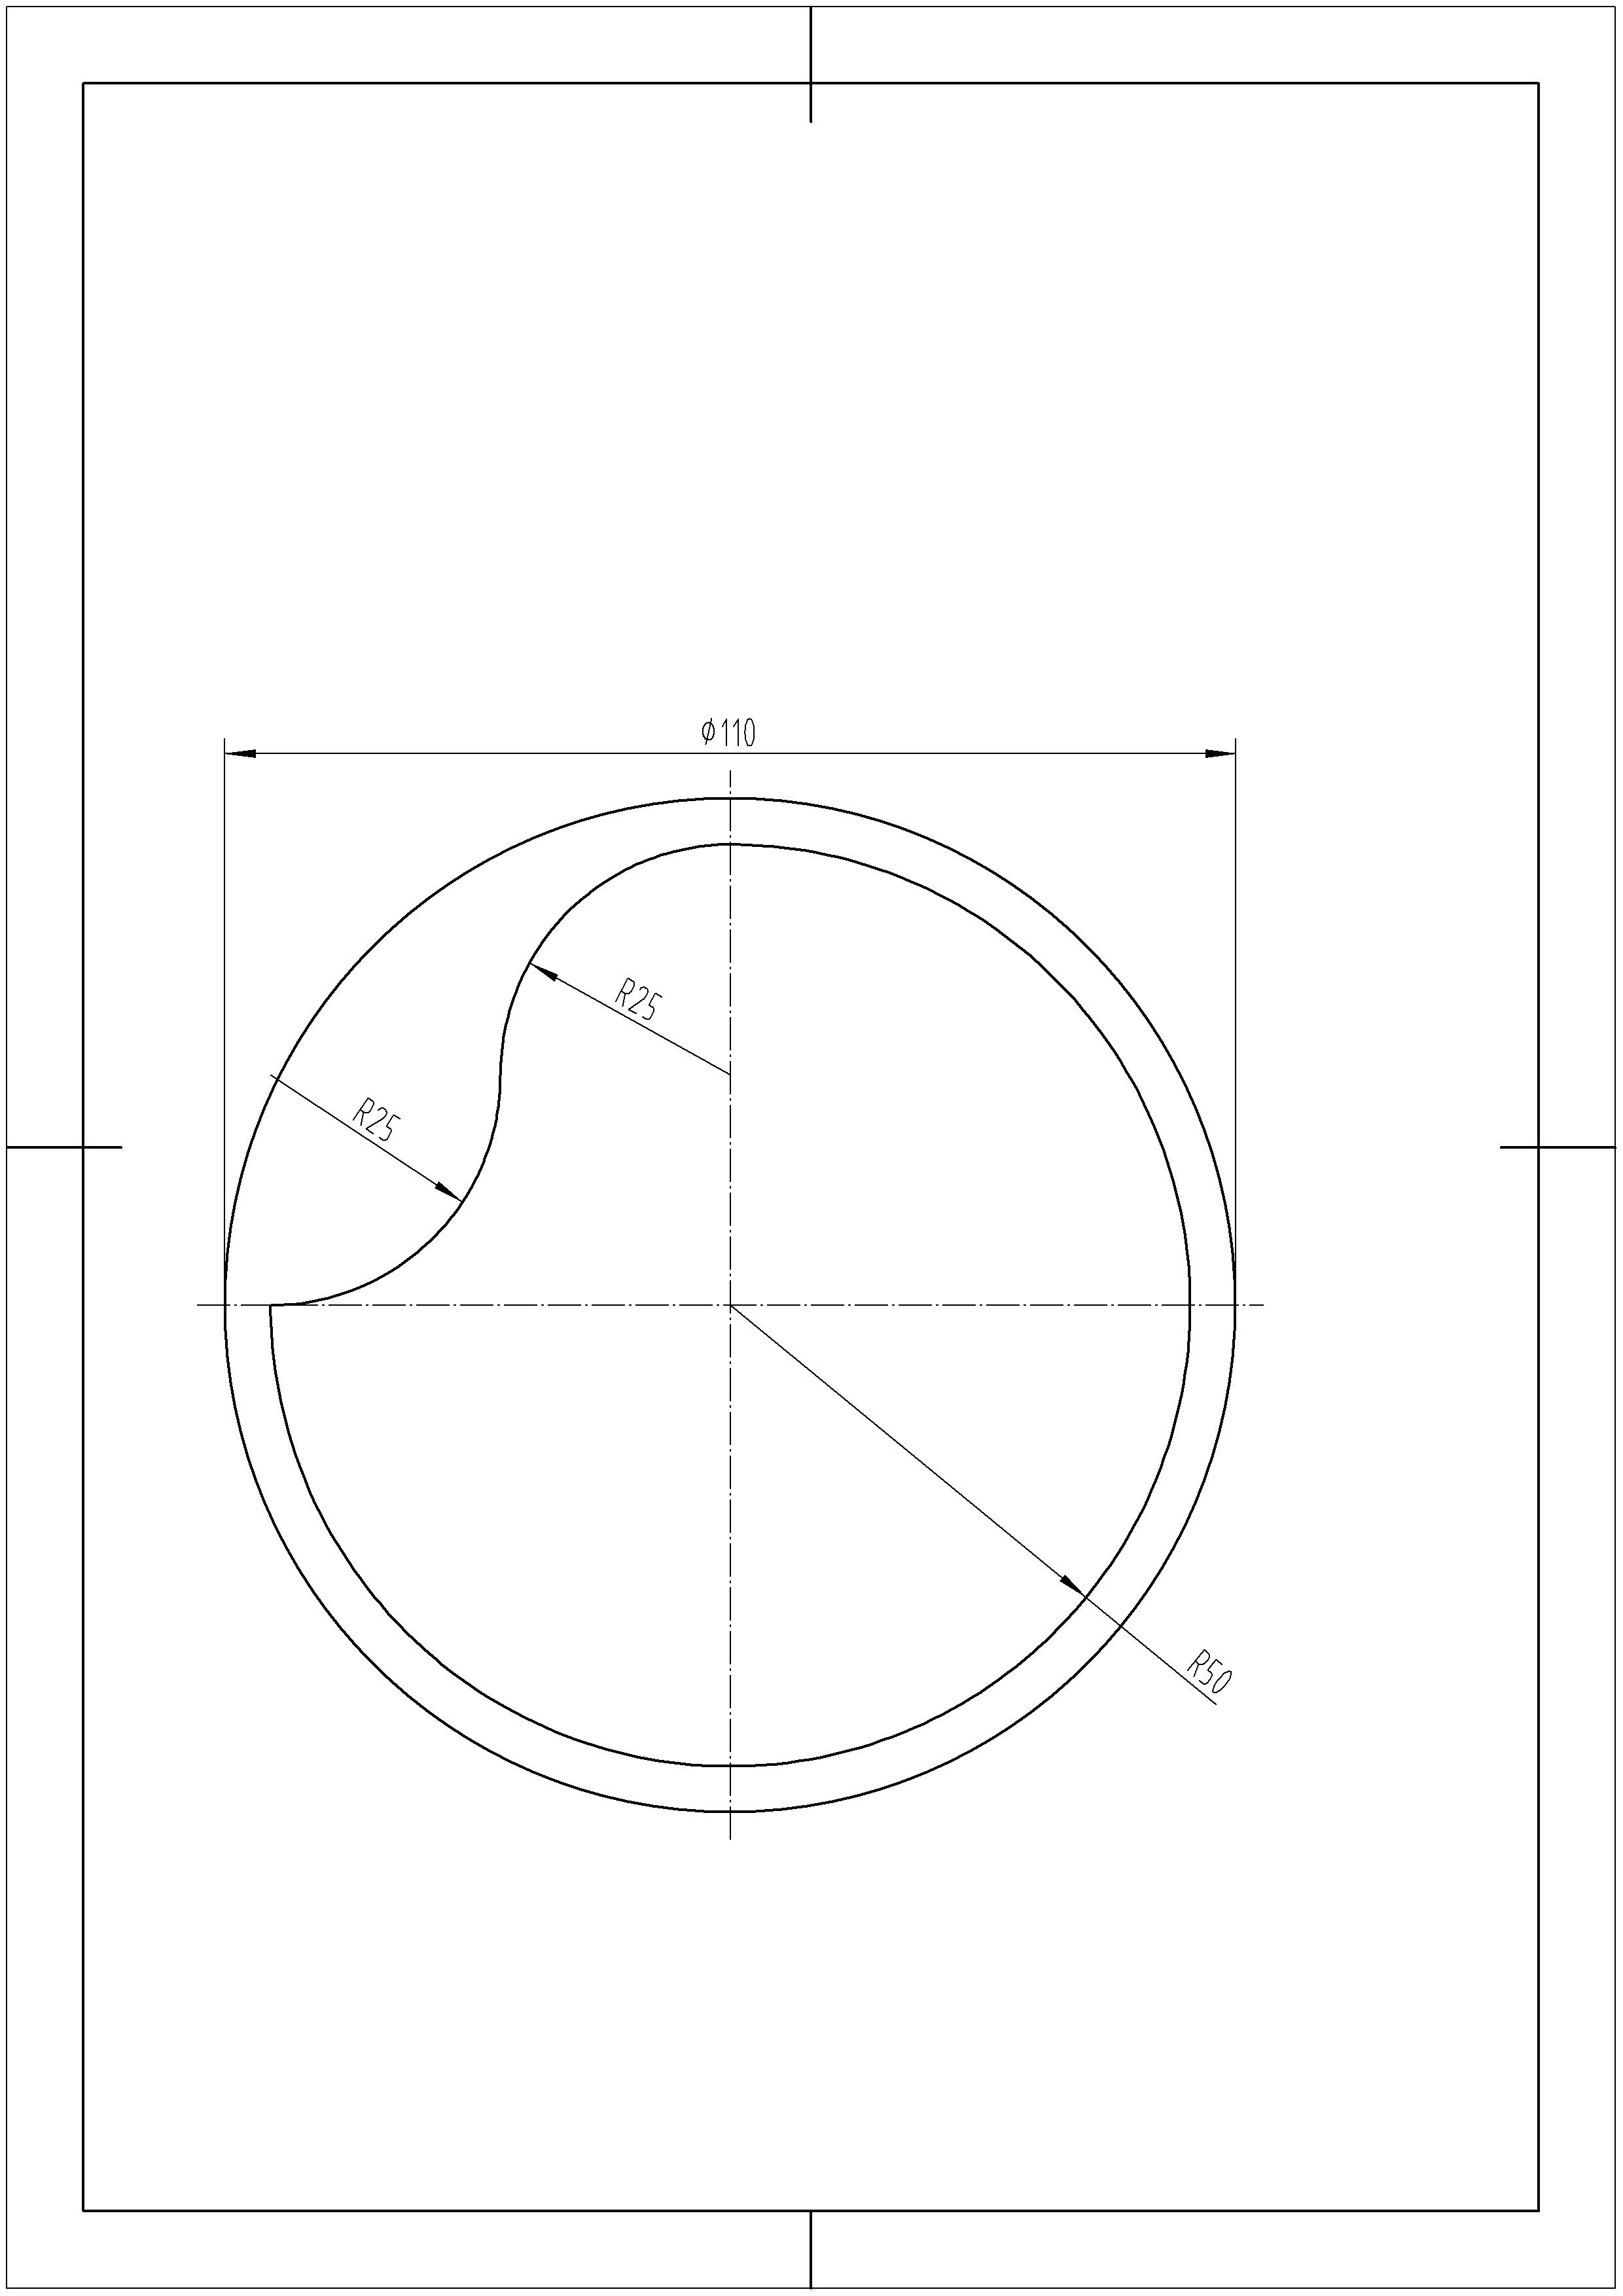
\includegraphics[width=0.8\linewidth,trim=40 150 70 220,clip]{data/image/7-1.jpg}
	\caption{刀补实例1}
	\label{fig:7-2}
\end{figure}

2、在数控铣床或加工中心上加工如图\ref{fig:7-3}所示的零件,试完成程序的编写。

\begin{figure}[h]
	\centering
	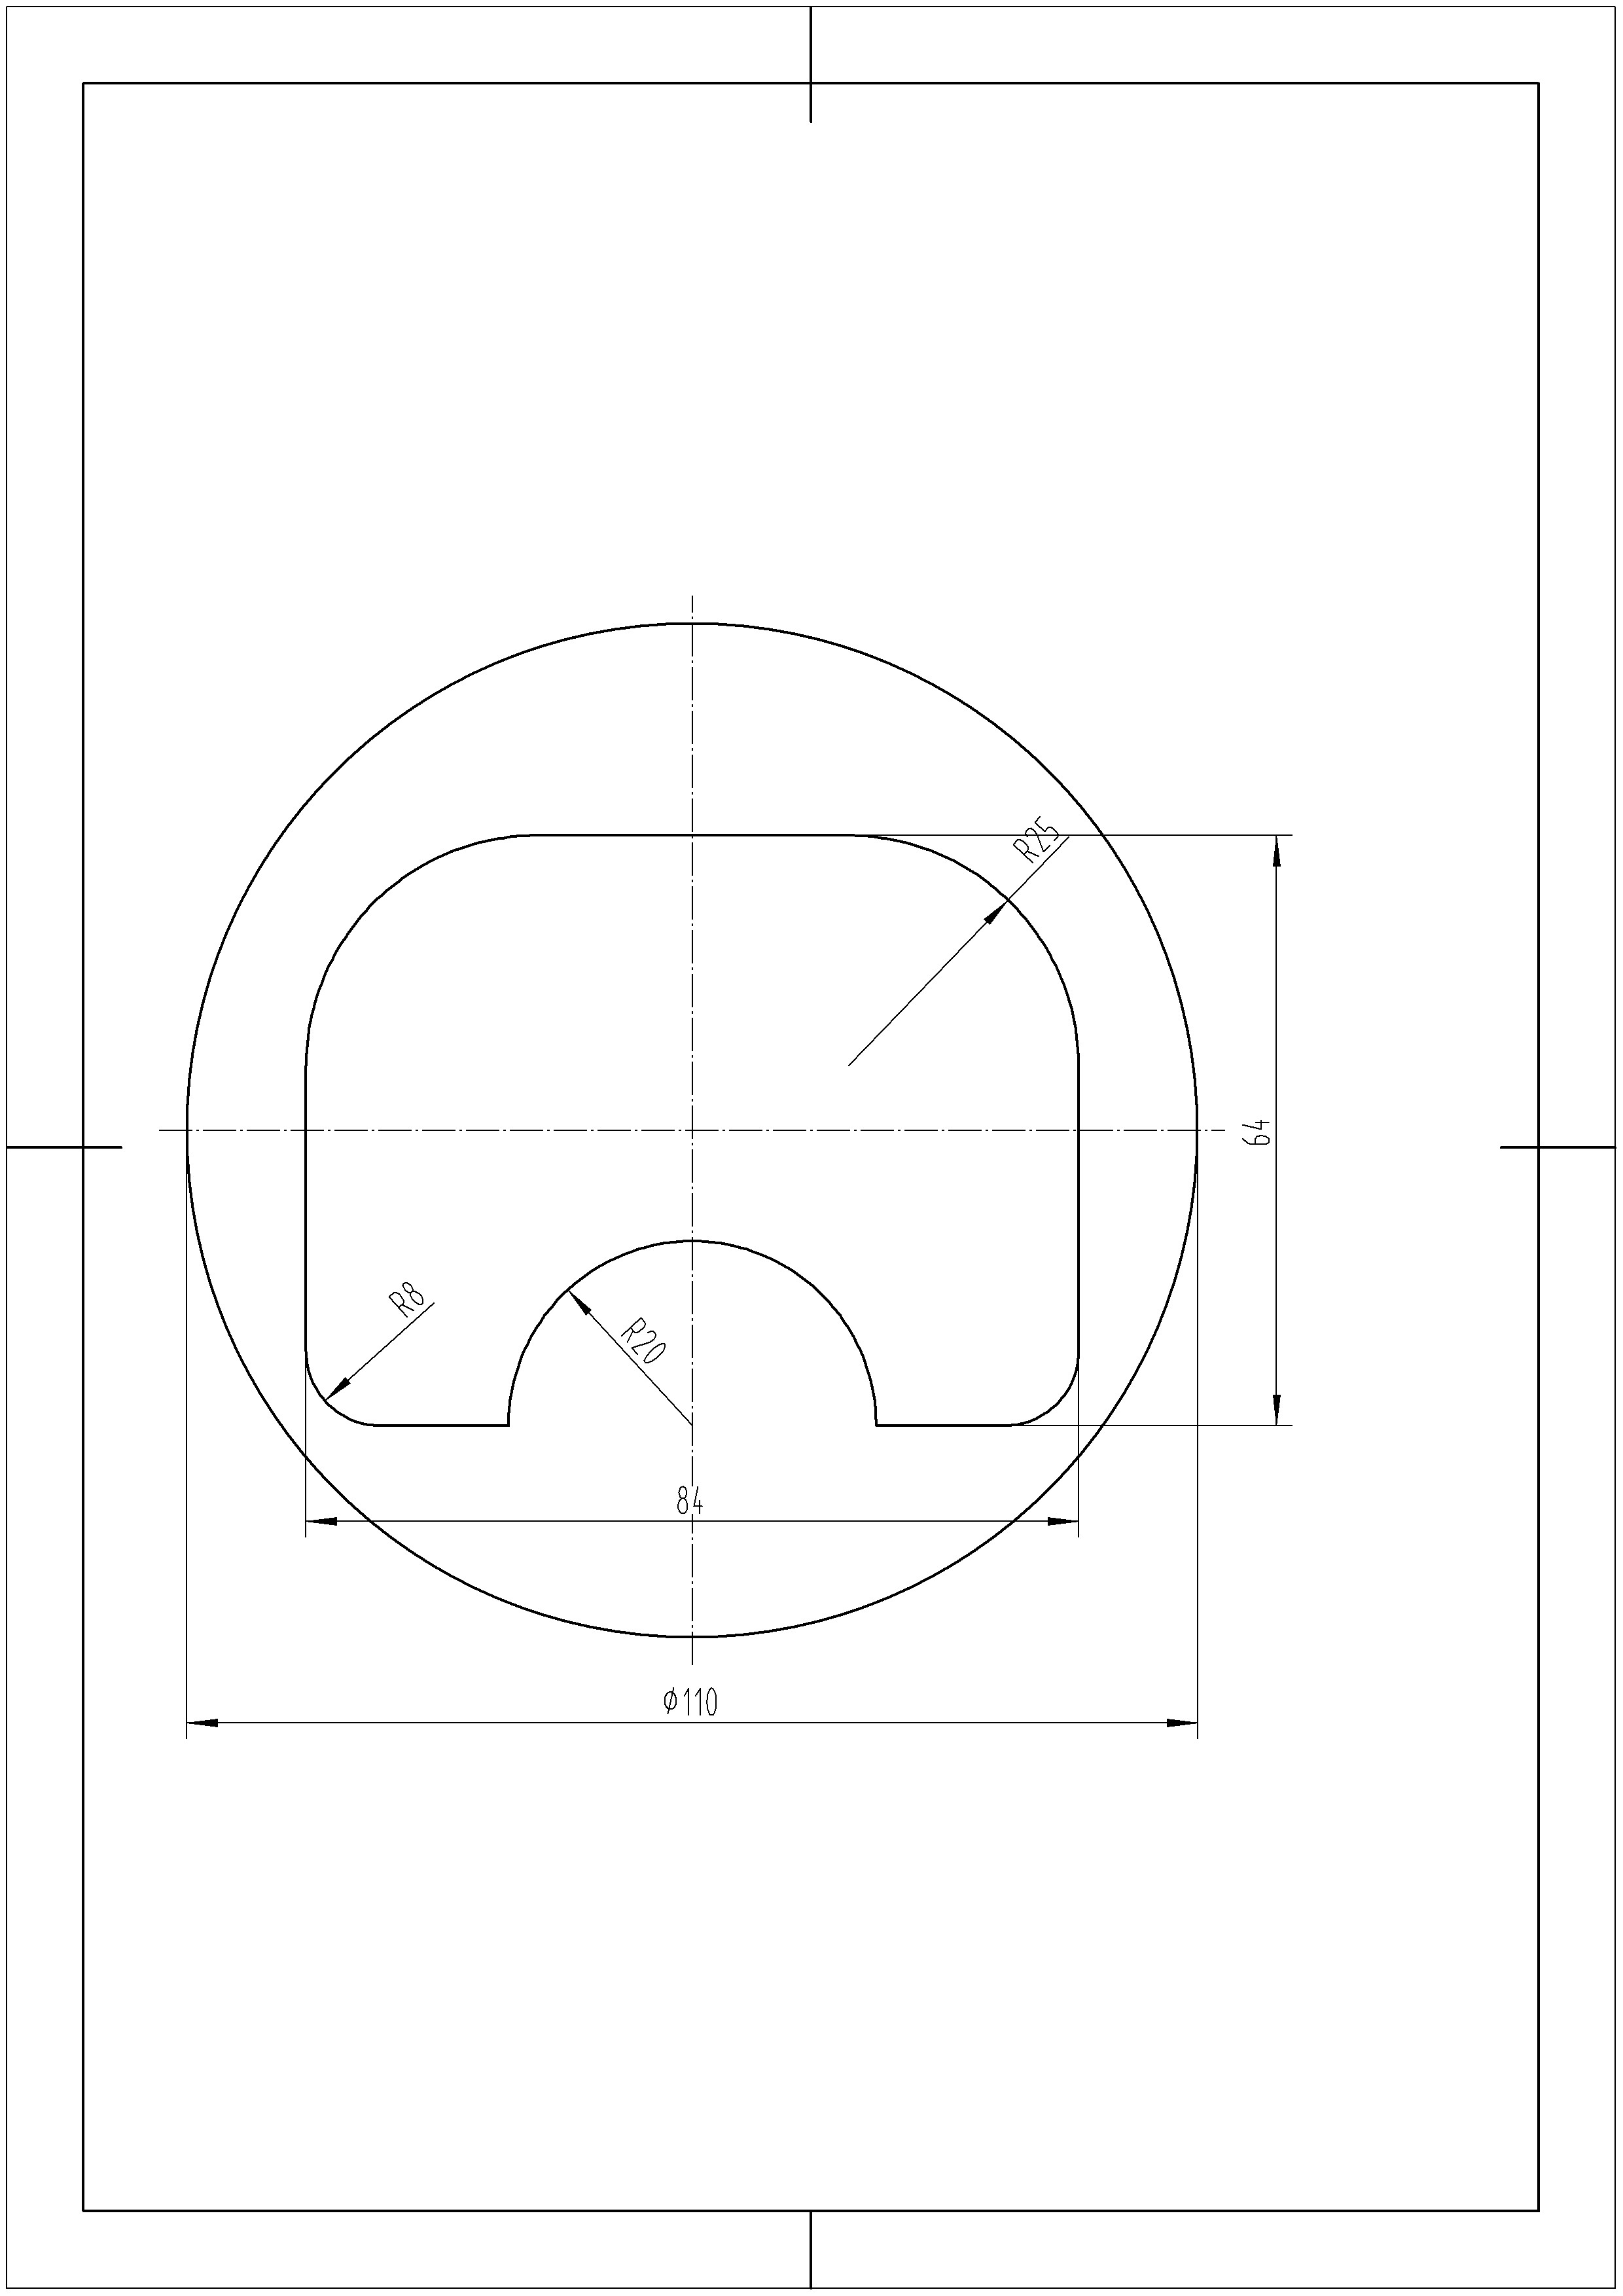
\includegraphics[width=0.8\linewidth,trim=40 150 70 220,clip]{data/image/7-2.jpg}
	\caption{刀补实例2}
	\label{fig:7-3}
\end{figure}


\subsection{课堂小结}
\begin{enumerate}[1、]
\item 刀补的概念
\item G40、G41/G42指令的使用;
\item 注意事项;
\item 刀补的编程;
\end{enumerate}

\vfill
\subsection{布置作业}
\begin{enumerate}[1、]
	\item 写出上面的程序。
	\item 习题集。
\end{enumerate}
\vfill